\documentclass[14pt, russian]{article}
\usepackage{graphicx}
\usepackage[a4paper,left=2.5cm,right=2.5cm,top=2.5cm,bottom=2.5cm]{geometry}%
\linespread{1.3}
\usepackage{amsbsy}
\usepackage{amssymb}
\usepackage{amsmath}
\usepackage[T2A]{fontenc}
\usepackage[cp1251]{inputenc}
\usepackage[russian]{babel}
\usepackage{epstopdf}
\usepackage[autostyle]{csquotes}
\usepackage{cuted}   
\usepackage{lipsum}  
\usepackage[intoc,nocfg,russian]{nomencl}
\newcommand{\nomencl}[2]{#1 --- #2\nomenclature{#1}{#2}}
\setlength{\nomlabelwidth}{3em}
\setlength{\nomitemsep}{-\parsep}
\setcounter{tocdepth}{2}
\renewcommand{\nomlabel}[1]{#1 ---}
\makenomenclature
\usepackage{wrapfig}
\let\vec=\mathbf
\def\mprp{\mbox{\tiny $\bot$}}
\def\mprl{\mbox{\tiny $\|$}}
\def\th{\mbox{th}}
\def\D{\mathrm{d}}
\def\beq{\begin{eqnarray}}
\def\eeq{\end{eqnarray}}
\def\ee{\varepsilon}
\def\lm{\lambda}
\newcommand{\ii}{\mathrm{i}} % мнимая единица
\newcommand{\dd}{\mathrm{d}} % дифференциал
\newcommand{\eee}{\mathrm{e}} % основание натуральных логарифмов

\newcommand{\bs}{\boldsymbol}

\begin{document}

%%%%%%%%%%%%%%%%%%%%%%%%%%%%%%%%%%%%%%%%%%%%%%%%%%%%%%%%%%%%%%%%%%%%%%%%

\title{Перенос излучения равновесной электронной плазмы с учетом резонансного комптоновского процесса.}
\author{Д.А. Румянцев, А.А. Ярков, Д.М. Шленев}
\date{}
\maketitle

% для заметок на полях
\marginparwidth = 2cm % ширина
%\renewcommand{\marginpar}[1]{} % отключить
\section{Введение}
Интерес к изучению комптоновского рассеяния $\gamma e \to \gamma e$ в 
сильном магнитном поле ($B\gtrsim B_e = m^2 / e= 4.41\cdot 10^{13}$ Гс~\footnote{В данной работе используется естественная система единиц: $c = \hbar = k_{\rm{B}} = 1$, $m$ -- масса электрона, $e > 0$ -- элементарный заряд.}) первоначально был вызван неожиданным открытием циклотронных 
спектральных линий у двойных рентгеновских 
пульсаров~\cite{Truemper1978,Makishima1990,Grove1995}, которые изначально 
интерпретировались либо как циклотронное поглощение, либо как циклотронное 
излучение~\cite{Truemper1978}. Дальнейшее повышение разрешения детекторов по 
энергии позволило уверенно заключить, что циклотронные особенности связаны 
именно с резонансным поглощением фотона~\cite{Mihara:1990}.
При этом под циклотронным резонансом обычно понимается 
резкое увеличение сечения рассеяния по сравнению с классическим томсоновским 
сечением, $\sigma_T = 8 \pi \alpha^2 /(3 m^2)$.
В представленных выше работах предполагалось, что начальный и конечные электроны находятся 
на основном уровне Ландау, тогда резонансные пики будут реализовываться при энергиях фотона~\cite{Daugherty:1986}:
\begin{equation}\label{eq:whn}
	\omega_n(\theta)= \frac{\sqrt{m^2+2 \beta n \sin^2\theta} - 
		m}{\sin^2\theta}\, ,
\end{equation}
где $\theta$ -- угол между импульсом начального фотона и направлением 
магнитного поля, $m$ -- масса электрона, $n=1,2,3...$ -- уровень Ландау виртуального электрона. 

В рассмотренных выше работах сечение комптоновского рассеяния 
становится бесконечным при энергиях фотона, соответствующих циклотронным 
резонансам~(\ref{eq:whn}) вследствие предположения о 
большом времени жизни виртуальных частиц. По этой причине их результаты 
справедливы только для областей энергий фотона вдали от резонансов
и могут быть применены, например, для моделирования излучения 
замагниченной 
холодной плазмы вблизи поверхности нейтронных 
звезд~\cite{Ozel:2001} или же для относительно слабых магнитных 
полей $B\lesssim 10^{10}$ Гс~\cite{Zavlin:1996}.

С другой стороны, учет резонансов в комптоновском процессе является необходимым 
при моделировании спектров излучения сильно замагниченных нейтронных 
звезд~\cite{Alexander:1991,Araya:1999,Ho:2001,Lyutikov:2006,Potekhin:2004,Schonherr:2007,Nishimura:2008,Suleimanov:2009}.
При этом вблизи поверхности нейтронной звезды, где формируется излучение, резонансный 
обратный комптоновский процесс рассеяния фотонов малых энергий на высокоэнергетических электронах 
является доминирующим процессом, который приводит к охлаждению плазмы 
внутренней магнитосферы и образованию высокоэнергетического хвоста в спектре 
излучения~\cite{Fernandez:2007,Nobili:2008,Baring:2018,Beloborodov:2013}.

Существует несколько основных способов решения задачи переноса излучения. Один из них заключается в решении системы интегро-дифференциальных уравнений, соответствующих системе уравнений Больцмана, составляемых для каждой компоненты среды. В работах~\cite{Nagel:1981,Kaminker:1982,Meszaros:1985,Alexander:1991,Nishimura:2008} для решения системы уравнений переноса использовался численный метод, который заключается в том, что интегрально-дифференциальные уравнения преобразуются в систему конечных разностей и квадратурных сумм с дискретизированными переменными, которая далее решается методом Фотрие~\cite{Mihalas:1985}.

 
С другой стороны, для численного анализа переноса излучения с учетом резонансного комптоновского процесса также активно используется метод Монте-Карло (см., например~\cite{Yahel:1979,Araya:1999,Nobili:2008,Fernandez:2011,Taverna:2014,Mustukov:2021,Mushtukov:2022}), который является достаточно мощным инструментом для моделирования сложных физических систем. Он заключается в использовании статистических подходов, связанных с генерацией псевдослучайных чисел, но имеет существенный недостаток, вызванный медленной сходимостью результата, поэтому для получения точных ответов требуется большое количество итераций, и, следовательно, более мощное оборудование~\cite{Caflisch:1998, Hall:2009}. Использование данного метода для моделировании поляризованного излучения в цилиндрической геометрии было начато еще в 70-х годах~\cite{Yahel:1979}. Основным преимуществом метода Монте-Карло является возможность с его помощью моделировать сложные физические процессы для случая сложных граничных условий или неоднородных сред. Так, в работе~\cite{Araya:1999} данный метод позволил рассматривать пространственную диффузию фотонов в произвольных геометриях с учетом углового распределения. Рентгеновское излучение, возникающего из-за резонансного комптоновсого рассеяния тепловых фотонов движущимися зарядами, в искривленной магнитосфере с помощью моделирования Монте-Карло изучалось в работе~\cite{Fernandez:2007}. Множественный комптоновский процесс рассматривался в работе \cite{Mushtukov:2022} в сильном магнитном поле, где в качестве результата было показано, что функция распределения фотонов с учетом циклотронных резонансов существенно отличается от равновесного распределения.

Из-за сложного поведения коэффициента поглощения фотона в комптоновском процессе вблизи резонанса задача переноса излучения становится нетривиальной. Одним из упрощений этой задачи является выбор геометрии излучающей области. Представление излучающей поверхности в виде бесконечной плиты является хорошим приближением для анализа излучения поверхности нейтронной звезды~\cite{Meszaros:1983,Harding:1984,Nishimura:2015}. С другой стороны, цилиндрическая геометрия является более подходящей для аккреционной колонки в целом~\cite{Basko:1976}. Согласно работе~\cite{Basko:1976}  под аккреционной колонкой понимается свободно падающее вещество "вмороженное" в линии магнитного поля вблизи полярных шапок и образующее некоторую воронку. Однако спектр, наблюдаемый в области циклотронных частот излучения аккрецирующих рентгеновских пульсаров, имеет более широкий профиль с заниженными значениями, чем рассчитанные с предположением данных геометрий. Поэтому в работе~\cite{Nishimura:2008} была предложена более подходящая модель формирования циклотронных линий, которая заключается в том, что результирующий спектр излучающей области формируется как сумма спектров от различных циклотронных областей, каждая из которых имеет цилиндрическую геометрию со своим постоянным значением плотности, температуры и индукции магнитного поля. Наконец, в работе~\cite{YarkovPhotFE:2023}, используя дельта-функциональное приближение было получено аналитическое решение кинетического уравнения для нахождения функции распределения фотонов двух возможных поляризаций в равновесной нерелятивистской плазме электронов в относительно сильном магнитном поле и с учетом резонанса на виртуальном электроне.

%%%%%%%%%%%%%%%%%%%%%%%%%%%%%%%%%%%%%%%%%%%%%%%%%%%%%%%%%%%%%%%%%%%%%%%%%%%%%%%%%%%%%%%%%%%%%%%%%%%%%%%%%%%%%%%%%%%%%%%%%%%%%%%%%%%%%%%%%%%%%%%%%%%%%%%%%%%
\section{Решение кинетического уравнения вблизи резонанса}

Следуя работе~\cite{YarkovPhotFE:2023} рассмотрим  достаточно узкую цилиндрическую колонку с осью, направленной вдоль магнитного поля (магнитное поле $B\lesssim B_e$ направлено вдоль оси~$z$), содержащую равновесную электронную плазму при температуре $T\ll m$. В точке $z=0$ этой колонки поддерживается стационарный поток фотонов с некоторой функцией распределения $f_{0\omega}^{(\lambda)}(x)$, где $\lambda=1,2$ -- поляризационные состояния фотонов. Для упрощения задачи предположим, что магнитное поле внутри колонки постоянно и однородно, а температура не зависит от координат и времени. В этом случае изменением функции распределения в направлении, поперечном к направлению магнитного поля можно пренебречь.

В силу нерелятивистского характера движения электронов в системе покоя плазмы, кинетическое уравнение Больцмана с учетом только парциальных процессов рассеяния фотонов на электронах можно записать в виде:
\begin{equation} 
\begin{aligned}\label{Kineq:Gen}
\frac{\partial f_\omega^{(\lambda)}(\xi, x)}{\partial \xi}&=\frac{1}{m}\sum_{\lambda'=1}^{2} \int dW_{\lambda\to\lambda'}\{f_{E'}(1-f_E)f^{(\lambda')}_{\omega'}(\xi, x') (1+f_\omega^{(\lambda)}(\xi, x))-
\\
&-f_E (1-f_{E'}) f_\omega^{(\lambda)}(\xi,x)(1+f^{(\lambda')}_{\omega'}(\xi, x'))
	\}\, .
\end{aligned}
\end{equation}

Здесь $\xi= m z$, $x = \cos \theta$, $x' = \cos \theta'$ ($\theta$ и $\theta'$ -- углы между направлениями импульсов начального и конечного фотона и направлением магнитного поля соответственно),   $f^{(\lambda)}_\omega(\xi, x)$ и $f^{(\lambda')}_{\omega'}(\xi, x')$ -- подлежащие определению функции распределения начального и конечного фотонов с энергиями $\omega$ и $ \omega'$ соответственно,  $f_E = 1/[\exp(E/T)+1]$ и $f_{E'} = 1/[\exp(E'/T)+1]$ --  равновесные функции распределения начального и конечного электронов с нулевым химическим потенциалом и энергиями начального и конечного электронов $E=\sqrt{p_z^2+M_\ell^2}$ и $E'=\sqrt{p_z^{\prime2}+M_{\ell \prime}^{ 2}}$ c соответствующими уровнями Ландау $\ell$ и $\ell'$, $dW_{\lambda \to \lambda'}$ -- коэффициент поглощения фотона~\cite{Rumyantsev:2017}:
%%%%%%%%%%%%%%%%%%%%%%%%%%%%%%%%
\beq
\label{eq:wabs1} 
&&W_{\gamma^{(1)} e \to \gamma e} = \frac{\alpha \beta}{2 \omega} 
\sum \limits^{\infty}_{\ell=0}  \sum \limits^{\infty}_{n=n_{0}} \sum \limits_{\epsilon = \pm 1} 
%\times 
%\\
%\nonumber
%&&\times 
\frac{f_{e}(E^{\epsilon}_{\ell}) [1 - f_{e}(E^{\epsilon}_{\ell} + 
\omega)]}{\sqrt{(M_n^2-M_{\ell}^2-q^{2}_{\mprl})^2-4 q^{2}_{\mprl}M_{\ell}^2}}
\times 
\\
\nonumber
&&\times 
\bigg \{ [2 \beta (n+\ell) - q^{2}_{\mprl}] (I^2_{n,\ell-1}+I^2_{n-1,\ell}) - 
%\\
%\nonumber
%&& -
8 \beta \sqrt{\ell n} I_{n,\ell-1} I_{n-1,\ell} \bigg \}   \, ,
\eeq
%
\beq
\label{eq:wabs2} 
&&W_{\gamma^{(2)} e \to \gamma e} = \frac{\alpha \beta}{2 \omega} 
\sum \limits^{\infty}_{\ell=0}  \sum \limits^{\infty}_{n=n_{0}} \sum \limits_{\epsilon = \pm 1} 
%\times 
%\\
%\nonumber
%&&\times 
\frac{f_{e}(E^{\epsilon}_{\ell}) [1 - f_{e}(E^{\epsilon}_{\ell} + 
\omega)]}{\sqrt{(M_n^2-M_{\ell}^2-q^{2}_{\mprl})^2-4 q^{2}_{\mprl}M_{\ell}^2}}
\times 
\\
\nonumber
&&\times 
\bigg \{ \left [\frac{(2\beta (n-\ell))^2}{q^{2}_{\mprl}} - 2 \beta (n+\ell) - 
4 m^2 \right ] 
%\times 
%\\
%\nonumber
%&& \times 
(I^2_{n,\ell}+I^2_{n-1,\ell-1}) %-
%\\
%\nonumber
%&&
-8 \beta \sqrt{\ell n} I_{n,\ell} I_{n-1,\ell-1} \bigg \}   \, ,
\eeq
где
\beq
\nonumber
&&E^{\epsilon}_{\ell} = \frac{1}{2 q^2_{\mprl}} \, \bigg [\omega \left (M^2_n - M^2_{\ell} - q^2_{\mprl} \right ) + 
\\
\nonumber
&&+\epsilon q_z 
\sqrt{\left (M^2_n - M^2_{\ell} - q^2_{\mprl} \right )^2 - 4 q^2_{\mprl} M^2_{\ell}} \, \bigg ] \, ,
\eeq
%
\noindent а также введена функция $I_{n, \ell}\equiv I_{n, \ell} \left(\frac{q_\perp^2}{2\beta}\right)$, которая для 
$n \geqslant \ell$ имеет следующий вид:
%
\begin{eqnarray}
	\nonumber
	&&I_{n, \ell} (x) = \sqrt{\frac{\ell !}{n !}} \; \eee^{-x/2} x^{(n-\ell)/2} L_\ell^{n-\ell} (x) \, ,
	\\
	&&I_{\ell, n} (x) = (-1)^{n-\ell} I_{n, \ell} (x) \, ,
	\label{eq:Inl}
\end{eqnarray}
\noindent где $L^k_n (x)$ -- обобщенные полиномы Лагерра~\cite{Gradstein:1963}. 
Отметим, что функция~(\ref{eq:Inl}) соответствуют функциям ${\Lambda}_{\ell, n} (x)$ в 
работах~\cite{Harding:1986,Gonthier:2014}.

 В~(\ref{eq:wabs1}) и~(\ref{eq:wabs2}) 
суммирование по $n$ ограничено согласно закону сохранения энергии и импульса следующим образом:  
%
\beq
n_0 = \ell + \left [\frac{q^2_{\mprl} + 2 M_\ell \sqrt{q^2_{\mprl}}}{2 \beta} \right ] \, , 
\eeq
\noindent где $[x]$ -- целая часть числа $x$.

%%%%%%%%%%%%%%%%%%%%%%%%%%%%%%%%%

Несмотря на то, что напряженность магнитного поля в данной задаче меньше критического значения $B\lesssim B_e$, начальный и конечный электроны преимущественно будут занимать основной уровень Ландау. Действительно, для параметров среды $B=10^{12}$ Гс и $T=5$ кэВ вклад высших уровней  по отношению к основному:

\begin{equation}
\begin{gathered}
\frac{\sum_{\ell=1}^{\infty}n_\ell}{n_0}\simeq 0.234 \, ,
\end{gathered}
\end{equation}
где
\begin{equation}
	n_\ell=\frac{\beta}{(2 \pi)^2} (2-\delta_{\ell,0}) \int \limits^{\infty}_{-\infty} \frac{\dd p_z}{\exp\left[\frac{1}{T}\sqrt{m^2+p_z^2+2\beta\ell}\right]+1}\, .
\end{equation}

Естественно ожидать, что при такой температуре электроны в плазме будут нерелятивистскими, поэтому в результате комптоновского процесса энергия начального фотона будет мало отличаться от энергии конечного фотона.
Таким образом, воспользовавшись методикой, развитой в работах~\cite{Kompaneets:1957,Lubarsky:1988}, правую часть уравнения (\ref{Kineq:Gen}) можно разложить по величине $\Delta\omega=\omega-\omega'\ll\omega$. Кроме того, будем пренебрегать индуцированным излучением так, что  $f_{\omega'}^{(\lambda')}(1+f_\omega^{(\lambda)})\simeq f_{\omega '}^{(\lambda')}$ и $f_\omega^{(\lambda)}(1+f^{(\lambda')}_{\omega'})\simeq f_\omega^{(\lambda)}$. В результате получим:
 
\begin{equation}\label{eq:KinSerDeltaw}
	\begin{aligned}
		&\frac{\partial f^{(\lambda)}_\omega(\xi,x)}{\partial \xi} = \frac{1}{x} \sum_{\lambda'=1}^{2} \int_{-1}^{1}dx'\varphi_\omega^{\lambda\lambda'}(x,x')\bigg\{ f^{(\lambda')}_{\omega}(\xi,x')-f^{(\lambda)}_\omega(\xi,x) -
		\\
		&-  
		\left[
		T \frac{\partial f_\omega^{(\lambda')}(\xi,x')}{\partial \omega} + f_\omega^{(\lambda')}(\xi,x')
		\right]\frac{\Delta \omega}{T}+
		\\
		&+ \frac{1}{2}  
		\bigg[
		T^2 \frac{\partial^2 f_\omega^{(\lambda')}(\xi,x')}{\partial \omega^2}+ 2T \frac{\partial f_\omega^{(\lambda')}(\xi,x')}{\partial \omega}+f_\omega^{(\lambda')}(\xi,x')
		\bigg]\left(\frac{\Delta\omega}{T}\right)^2\bigg\}
		\,  ,
	\end{aligned}
\end{equation}
где
\begin{equation}
	\varphi^{\lambda \lambda'}_\omega(x,x') = 
	\frac{n_e \omega'}{32 \pi m \omega} \sum_{s''=\pm 1} \int\limits_{0}^{2\pi}\frac{\dd\varphi'}{2\pi} \frac{\left|{\cal M}^{s''}_{e_1\to e_0 \gamma^{(\lambda ')}}\right|^2\left|{\cal M}^{s''}_{ e_0 \gamma^{(\lambda)}\to e_1}\right|^2}
	{(\omega^2 (1-x^2)+ 2\omega m - 2\beta)^2 + (\Gamma_1^{s''} E_n''/2)^2}
\end{equation}
где амплитуда поглощения фотона может быть представлена в виде~\cite{Rumyantsev:2017}:
%
\begin{eqnarray}
	\label{eq:amplonever} 
	&&{\cal M}^{s'' s}_{\gamma^{(\lambda)} e_\ell \to e_n} =  \frac{\exp{[-\ii q_x (p_y + p_y^{\,\prime \prime})/(2\beta)]}}{\sqrt{M_{\ell} M_n (M_{\ell} + m) 
			(M_n + m)}} 
	\times
	\nonumber\\[3mm]
	&&\times 
	\left [ \frac{q_y+\ii q_x}{\sqrt{q_{\mprp}^2}} \right ]^{n-\ell} {\cal T}^{s'' s}_\lambda \, .
\end{eqnarray}

Величины ${\cal T}^{s'' s}_\lambda$, входящие в выражение~(\ref{eq:amplonever}), приводятся в Приложении 1.

Из закона сохранения энергии и $z$-компоненты импульса в реакции  $\gamma e \to \gamma e$  найдем:
\begin{equation}
\begin{aligned}
\omega'=\frac{1}{1-x'^2}\left\{E- p_z x'+\omega(1- x x')-\sqrt{\left[E-p_z x'+\omega(1- x x')\right]^2-2\beta\left(1-x'^2\right)}\right\}.
\end{aligned}
\end{equation}


Функции $\varphi_\omega^{\lambda\lambda'}(x,x')$ могут быть получены из результатов работы~\cite{Rumyantsev:2017} и в случае, когда масса электрона является максимальным параметром задачи, будут иметь следующий вид:
\begin{equation}\label{eq:Varphi}
\begin{aligned}
&\varphi_\omega^{11}(x,x')\simeq \rho m^3 \left(\frac{\beta^2}{\Delta^-} +\frac{\left[m \omega -\beta\right]^2}{\Delta^+}\right)\, ,
\\
&\varphi_\omega^{12}(x,x')\simeq \rho \omega^2 m^3 \left(
\frac{x'^2 m^2}{\Delta^-} + \frac{\left[m\omega - \beta\right]}{2 \Delta^+}
\right)	\, ,
\\
&
\varphi_\omega^{22}(x,x')\simeq \rho \omega^4 m^3
\left(
\frac{m^4x^2 x'^2 }{\beta^2 \Delta^-} + \frac{1}{4\Delta^+}
\right)\, ,
\\
&
\varphi_\omega^{21}(x,x')\simeq \rho \omega^2 m^3
\left(
\frac{m^2 x^2}{\Delta^-} + \frac{[m\omega - \beta]}{2 \Delta^+}
\right)\, ,
\end{aligned}
\end{equation}
где
\begin{equation}
\rho = \frac{n_e}{8\pi} e^4 \left(\frac{\sqrt{m^2+2\beta} + m}{\sqrt{m^2+2\beta}}\right)\simeq \frac{n_e}{4\pi}e^4\, ,
\end{equation}

\begin{equation}
\Delta^\pm = \left[\omega^2(1-x^2)+2 \omega m - 2\beta\right]^2 + \left(\frac{E_1{''} \Gamma^\pm_1}{2}\right)^2 \, ,
\end{equation}
$\Gamma^\pm_1$ -- полная ширина поглощения электрона, находящегося на первом уровне Ландау, для двух возможных поляризационных состояний электрона.  Она может быть получена из результатов работы~\cite{Kuznetsov:2003} и представлена в следующем виде:
\begin{equation}
E_1''\Gamma_1^{\pm} \simeq \frac{e^2\beta^2}{\pi M_1}\frac{1}{M_1\pm m} \int_{0}^{\zeta}\dd x e^{-x} \frac{1-\zeta x}{\sqrt{x^2-\zeta x+1}},
\end{equation}
где $M_1=\sqrt{m^2+2\beta}\simeq m$, $\zeta=(M_1^2+m^2)/\beta\simeq 2m^2/\beta$,

Уравнение~(\ref{eq:KinSerDeltaw}) относительно переменной $\xi$ удобно представить в виде:
\begin{equation}\label{eq:GenSolve}
	\frac{\partial f^{(\lambda)}_\omega(\xi,x)}{\partial \xi} =
	-{\cal \chi}_\omega^{(\lambda)}(x) f^{(\lambda)}_\omega(\xi,x) + F^{(\lambda)}_\omega(\xi,x),
\end{equation}
где 
\begin{equation}
	{\cal \chi}_\omega^{(\lambda)}(x) = \frac{1}{x} \int_{-1}^{1} \dd x' \left\{\varphi^{\lambda 1}_\omega(x,x')+\varphi^{\lambda 2}_\omega(x,x')\right\}\, ,
\end{equation}

\begin{equation}
	\begin{aligned}
		&F_\omega^{(\lambda)}(\xi,x)= \frac{1}{x} \sum_{\lambda'=1}^{2}\int_{-1}^{1}\dd x' \varphi_\omega^{\lambda\lambda'}(x,x')\bigg\{  f^{(\lambda')}_{\omega}(\xi,x') -
		\\
		&-  
		\left[
		T \frac{\partial f_\omega^{(\lambda')}(\xi,x')}{\partial \omega} + f_\omega^{(\lambda')}(\xi,x')
		\right]\frac{\Delta \omega}{T}+
		\\
		&+ \frac{1}{2}  
		\bigg[
		T^2 \frac{\partial^2 f_\omega^{(\lambda')}(\xi,x')}{\partial \omega^2}+ 2T \frac{\partial f_\omega^{(\lambda')}(\xi,x')}{\partial \omega}+f_\omega^{(\lambda')}(\xi,x')
		\bigg]\left(\frac{\Delta\omega}{T}\right)^2\bigg\}
		\,  .
	\end{aligned}
\end{equation}

Решение уравнения~(\ref{eq:GenSolve}) с учетом граничных условий на функцию распределения
можно представить в следующем виде:
\begin{equation}
	f^{(\lambda)}_\omega(\xi,x)= f^{(\lambda)}_{0\omega}(x) e^{-{\cal \chi}_\omega^{(\lambda)}(x)\xi}+\int_{0}^{\xi}\dd \xi' e^{-{\cal \chi}_\omega^{(\lambda)}(x)(\xi-\xi')} F_\omega^{(\lambda)}(\xi',x)\, .
\end{equation}

Далее будем полагать, что в точке $z=0$ поддерживается стационарный поток фотонов двух мод описываемый изотропной функцией распределения:
\begin{equation}\label{eq:GranS}
f^{(\lambda)}_{0\omega}(x)=f_{0\omega} \, .
\end{equation}

В результате, уравнение (\ref{eq:KinSerDeltaw}) перепишем следующим образом:
\begin{equation}\label{FormSol}
\begin{aligned}
&f_\omega^{(\lambda)}(\xi,x)=f_{0\omega} 	e^{-{\cal \chi}_\omega^{(\lambda)}(x)\cdot \xi} + \frac{1}{x}\int_{0}^{\xi}d\xi'\int_{-1}^{1}dx' e^{-{\cal \chi}_\omega^{(\lambda)}(x)\cdot (\xi-\xi')}\times 
\\
&\times\sum_{\lambda'=1}^2\varphi_\omega^{\lambda 	\lambda'}(x,x')\bigg\{f_\omega^{(\lambda')}(\xi',x') - \frac{\Delta \omega}{T}
\left[
T \frac{\partial f_\omega^{(\lambda')}(\xi',x')}{\partial \omega} + f_\omega^{(\lambda')}(\xi',x')
\right]+
\\
&+ \frac{1}{2}\left(\frac{\Delta \omega}{T}\right)^2
\left[
T^2 \frac{\partial^2 f_\omega^{(\lambda')}(\xi',x')}{\partial \omega^2} + 2T \frac{\partial f_\omega^{(\lambda')}(\xi',x')}{\partial \omega}+f_\omega^{(\lambda')}(\xi',x')
\right]\bigg\}\, .
\end{aligned}	
\end{equation}


Далее разложим функцию распределения фотонов по полиномам Лежандра ${\cal P}_\ell(x)$~\cite{Gradstein:1963} относительно переменной $x$:

\begin{equation}\label{eq:fSerLegender}
f_\omega^{(\lambda)}(\xi, x) = \sum_{\ell = 0}^{\infty} A_\ell^{(\lambda)}(\xi,\omega) {\cal P}_\ell(x)\, ,
\end{equation}

Подставляя (\ref{eq:fSerLegender}) в (\ref{FormSol}) и применяя к полученному выражению преобразование Лапласа относительно переменной $\xi$, получим систему дифференциальных уравнений второго порядка на коэффициенты $A_\ell^{(\lambda)}(\xi,\omega)$ относительно переменной $\omega$:
\begin{equation}\label{eq:SysEqALapX}
\begin{aligned}
&\sum_{\ell' = 0}^{\infty} \overline{A}_{\ell'}^{(\lambda)}(s,\omega) {\cal P}_{\ell'}(x) = \frac{f_{0\omega} }{s+{\cal \chi}^{(\lambda)}_\omega(x)}+
\sum_{\ell'=0}^{\infty}\int_{-1}^{1}\dd x'\frac{1}{x} \frac{{\cal P}_{\ell'}(x')}{s+{\cal \chi}_\omega^{(\lambda)}(x)} \times
\\
&\times\sum_{\lambda'=1}^2\varphi_\omega^{\lambda\lambda'}(x,x')\bigg\{ \overline{A}_{\ell'}^{(\lambda')}(s,\omega) - \frac{\Delta \omega}{T}
\left[
T \frac{\partial \overline{A}_{\ell'}^{(\lambda')}(s,\omega)}{\partial \omega} + \overline{A}_{\ell'}^{(\lambda')}(s,\omega)
\right]+
\\
&+ \frac{1}{2}\left(\frac{\Delta \omega}{T}\right)^2
\left[
T^2 \frac{\partial^2 \overline{A}_{\ell'}^{(\lambda')}(s,\omega)}{\partial \omega^2} + 2T \frac{\partial \overline{A}_{\ell'}^{(\lambda')}(s,\omega)}{\partial \omega}+\overline{A}_{\ell'}^{(\lambda')}(s,\omega)
\right]\bigg\}\, ,
\end{aligned}
\end{equation}
где 

\begin{equation}\label{lapA}
\overline{A}_{\ell'}^{(\lambda)}(s,\omega)=\int_{0}^{\infty} A^{(\lambda)}_{\ell'}(\xi,\omega) e^{-s\xi}d\xi\, .
\end{equation}

Домножая обе части выражения~(\ref{eq:SysEqALapX}) на ${\cal P}_\ell(x)$, проинтегрируем его по~$x$. С учетом
ортогональности полиномов Лежандра:

\begin{equation}
\int_{-1}^{1}\dd x {\cal P}_\ell(x) {\cal P}_{\ell'}(x)=\frac{2}{2\ell+1}\delta_{\ell \ell'}\, ,
\end{equation}
окончательно получим следующую систему уравнений для нахождения коэффициентов $\overline{A}_\ell^{(\lambda)}(s,\omega)$:

\begin{equation}\label{eq:SysEqALap}
\begin{aligned}
\frac{2}{2 \ell +1} &\overline{A}_\ell^{(\lambda)}(s,\omega) = \int_{-1}^{1} \frac{f_{0\omega}}{s+{\cal \chi}^{(\lambda)}_\omega(x)}{\cal P}_\ell(x)\dd x+
\sum_{\ell'=0}^{\infty}\int_{-1}^{1}\dd x'\int_{-1}^{1}\frac{\dd x}{x} \frac{{\cal P}_\ell(x) {\cal P}_{\ell'}(x')}{s+{\cal \chi}_\omega^{(\lambda)}(x)} \times
\\
&\times\sum_{\lambda'=1}^2\varphi_\omega^{\lambda\lambda'}(x,x')\bigg\{ \overline{A}_{\ell'}^{(\lambda')}(s,\omega) - \frac{\Delta \omega}{T}
\left[
T \frac{\partial \overline{A}_{\ell'}^{(\lambda')}(s,\omega)}{\partial \omega} + \overline{A}_{\ell'}^{(\lambda')}(s,\omega)
\right]+
\\
&+ \frac{1}{2}\left(\frac{\Delta \omega}{T}\right)^2
\left[
T^2 \frac{\partial^2 \overline{A}_{\ell'}^{(\lambda')}(s,\omega)}{\partial \omega^2} + 2T \frac{\partial \overline{A}_{\ell'}^{(\lambda')}(s,\omega)}{\partial \omega}+\overline{A}_{\ell'}^{(\lambda')}(s,\omega)
\right]\bigg\}\, .
\end{aligned}
\end{equation}

Далее, подставляя функции~(\ref{eq:Varphi}) в~(\ref{eq:SysEqALap}) и интегрируя получившийся результат по $x'$, с учетом $\Delta\omega\simeq \omega -\beta/m$ получим следующую бесконечную  систему зацепляющихся уравнений для нахождения коэффициентов $\overline{A}_\ell^{(\lambda)}(s,\omega)$:

\begin{equation}\label{eq:SysAPart}
\begin{aligned}		
\frac{2}{2 \ell +1} &\overline{A}_\ell^{(\lambda)}(s,\omega)= f_{0\omega} {\cal J}_\ell^{(\lambda)}(s,\omega) +
\\
&+2J_\ell^{\lambda 1}(s,\omega)\bigg\{ \overline{A}_{0}^{(1)}(s,\omega) - \frac{\Delta\omega}{T} 
\left[
T \frac{\partial \overline{A}_{0}^{(1)}(s,\omega)}{\partial \omega} + \overline{A}_{0}^{(1)}(s,\omega)
\right]+
\\
&+ \frac{1}{2}\left(\frac{\Delta\omega}{T}\right)^2 
\left[
T^2 \frac{\partial^2 \overline{A}_{0}^{(1)}(s,\omega)}{\partial \omega^2} + 2T \frac{\partial \overline{A}_{0}^{(1)}(s,\omega)}{\partial \omega}+\overline{A}_{0}^{(1)}(s,\omega)
\right]\bigg\}+
\\
&+\frac{2}{3} J_\ell^{\lambda 2}(s,\omega)\bigg\{\overline{A}_{0}^{(2)}(s,\omega) - \frac{\Delta\omega}{T} 
\left[
T \frac{\partial \overline{A}_{0}^{(2)}(s,\omega)}{\partial \omega} + \overline{A}_{0}^{(2)}(s,\omega)
\right]+
\\
&+ \frac{1}{2}\left(\frac{\Delta\omega}{T}\right)^2 
\left[
T^2 \frac{\partial^2 \overline{A}_{0}^{(2)}(s,\omega)}{\partial \omega^2} + 2T \frac{\partial \overline{A}_{0}^{(2)}(s,\omega)}{\partial \omega}+\overline{A}_{0}^{(2)}(s,\omega)
\right]\bigg\}+
\\
&+\frac{4}{15}J_\ell^{\lambda 2}(s,\omega)\bigg\{\overline{A}_{2}^{(2)}(s,\omega) - \frac{\Delta\omega}{T} 
\left[
T \frac{\partial \overline{A}_{2}^{(2)}(s,\omega)}{\partial \omega} + \overline{A}_{2}^{(2)}(s,\omega)
\right]+
\\
&+ \frac{1}{2}\left(\frac{\Delta\omega}{T}\right)^2 
\left[
T^2 \frac{\partial^2 \overline{A}_{2}^{(2)}(s,\omega)}{\partial \omega^2} + 2T \frac{\partial \overline{A}_{2}^{(2)}(s,\omega)}{\partial \omega}+\overline{A}_{2}^{(2)}(s,\omega)
\right]\bigg\}\, ,
\end{aligned}
\end{equation}
где 
\begin{equation}\label{eq:J01}
{\cal J}_\ell^{(\lambda)}(s,\omega)=\int_{-1}^{1} \frac{{\cal P}_\ell(x)\dd x}{s+{\cal \chi}^{(\lambda)}_\omega(x)},
\end{equation}

\begin{equation}\label{eq:Jll}
J_\ell^{\lambda\lambda'}(s,\omega) =\int_{-1}^{1}\dd x'\int_{-1}^{1}\dd x \frac{1}{x} \frac{{\cal P}_\ell(x)}{s+\chi_\omega^{(\lambda)}(x)} \varphi^{\lambda \lambda '}_\omega(x,x')\, .
\end{equation}

Отметим, что в правую часть системы уравнений (\ref{eq:SysAPart}) входят лишь   коэффициенты $\overline{A}_0^{(1)}(s,\omega)$, $\overline{A}_0^{(2)}(s,\omega)$, $\overline{A}_2^{(2)}(s,\omega)$, поэтому для построения рекурентного соотношения, позволяющего определить все коэффициенты $\overline{A}_n^{(\lambda)}(s,\omega)$, необходимо решить лишь систему из трех дифференциальных уравнений. 

Найденные таким образом коэффициенты $\overline{A}_\ell^{(\lambda)}(s,\omega)$  из системы (\ref{eq:SysAPart}) с учетом~(\ref{eq:J01})--(\ref{eq:Jll})
 позволяют  решить задачу о расчете функции распределения фотонов в терминах образов по Лапласу по переменной $\xi$. После применения обратного преобразования Лапласа окончательно функцию распределения фотонов поляризации~$\lambda$ можно представить в следующем виде:
\begin{equation}\label{eq:SolveFunc}
f_\omega^{(\lambda)}(z, x) = \frac{1}{2\pi i}\sum_{\ell=0}^{\infty} 
{\cal P}_\ell(x)\int_{\sigma_c-i\infty}^{\sigma_c + i \infty}ds \cdot e^{s\xi} \overline{A}^{(\lambda)}_\ell(s,\omega)\, ,
\end{equation}
где интеграл берется в комплексной плоскости по прямой $\text{Re} \, s = \sigma_c$.
%%%%%%%%%%%%%%%%%%%%%%%%%%%%%%%%%%%%%%%%%%%%%%%%%%%%%%%%%%%%%%%%%%%%%%%%%%%%%%%%%%%%%%%%%%%%%%%%%%%%%%%%%%%%%%%%%%%%%%%%%%%%%%%%%%%%%%%%%%%%%%%%%%%%%%%%%%%
\section{Численный анализ}

Для сравнения полученного решения с результатами численного моделирования Монте-Карло, рассмотрим решение кинетического уравнения при значениях магнитного поля $B=0.05 B_e$, температуры $T=3$ кэВ и концентрации $n_e\simeq 10^{11} \text{ см}^{-3}$.
Следует отметить, что в при таких условиях коэффициент $J_\ell^{\lambda\lambda'}(s,\omega)$ во много меньше ${\cal J}_\ell^{(\lambda)}(s,\omega)$ в ветвях резонанса, поэтому коэффициенты разложения по полиномам Лежандра можно определить достаточно простым образом:
\begin{equation}
	\frac{2}{2 \ell +1} \overline{A}_\ell^{(\lambda)}(s,\omega)= f_{0\omega} {\cal J}_\ell^{(\lambda)}(s,\omega),
\end{equation}
что приводит к очень простому результату, который может быть получен также из выражения~(\ref{FormSol}):
\begin{equation}\label{FormSolZeroL}
	f_\omega^{(\lambda)}(\xi,x)=f_{0\omega} 	e^{-{\cal \chi}_\omega^{(\lambda)}(x)\cdot \xi}.
\end{equation}

 Будем полагать, что в отсутствии влияния резонансного комптоновского процесса, функция распределения описывается степенным законом с экспоненциальным подавлением высоких энергий~\cite{Schonherr:2007,Araya:1999,SandeepK:2022,Nishimura:2015}:
\begin{equation}\label{eq:functionZerof}
	f_{0\omega} = A\omega^{-\alpha} \exp(-\omega/\omega_f),
\end{equation}
где $A$ -- нормировочный множитель, $\alpha$ -- спектральный индекс фотона,   $\omega_f$ -- энергия подавления. Функция распределения~(\ref{eq:functionZerof})  является простейшей моделью для описания спектра рентгеновских пульсаров, которая хорошо подходит для демонстрации влияния резонансного комптоновского рассеяния.

Далее для описания переноса излучения в среде удобно использовать характеристику, называемую оптической толщой:
\begin{equation}
	\tau = \int_0^z W_{\gamma^{(\lambda)} e \to \gamma^{(\lambda')} e} d\ell,
\end{equation}	
которая, строго говоря зависит от энергии начального фотона, от углов между импульсом начального (конечного) фотона и направлением магнитного поля. 
	В случае однородной среды для среднего значения оптической толщи получим:
\begin{equation}
	\tau = z /\ell_\lambda,
\end{equation}
	где $z$ -- геометрический путь луча, $\ell_\lambda$ -- средняя длина свободного пробега фотона моды $\lambda$, которая в случае доминирующего комптоновского процесса может быть оценена, как среднее по Росселанду следующим образом:
	\begin{equation}\label{eq:l}
		\ell_\lambda =\sum_{\lambda'= 1,2} \frac{\int_0^{\infty} W^{-1}_{\gamma^{(\lambda)} e \to \gamma^{(\lambda')} e} \frac{\partial f_\omega^{(\lambda')}(x,z)}{\partial T} \frac{d^3k}{(2\pi)^3}}{\int_0^\infty\frac{\partial f^{(\lambda')}_\omega(x,z)}{\partial T} \frac{d^3k}{(2\pi)^3}},
	\end{equation}

Анализ выражения~(\ref{eq:l}) в приближении $f^{(\lambda')}_\omega=f_{0\omega}$ с учетом~(\ref{FormSolZeroL}) дает:
\begin{equation}
	\tau\simeq \frac{2 z \rho \beta^2}{m^6}
\end{equation}

На рис.~\ref{fig:Mode11tau}--\ref{fig:Mode22tau} представлены функции распределения для моды 1 и 2 при различных значениях оптической толщи (\mbox{$\tau_{1}=3\times 10^{-4}$} и $\tau_{2}=3\times 10^{-3}$) и концентрации электронов $n_e = 10^{12}$ см$^{-3}$ в~приближении~(\ref{FormSolZeroL}), которые сравниваются с  функциями распределения фотонов, полученными в~результате моделирования циклотронных линий для аккрецирующееся цилиндрической колонки вещества методом Монте-Карло~\cite{Schonherr:2007}. Как видно из представленных результатов на рис.~\ref{fig:Mode11tau} для фотона моды 1 имеется существенное влияние угла $\theta$ между импульсом фотона и направлением магнитного поля на ширину резонансного пика. В приближении~(\ref{FormSolZeroL}) наблюдаются значительные провалы в резонансных областях, связанных с резонансным поведением функций ${\cal \chi}_\omega^{(\lambda)}(x)$ и соответствующих разным уровням Ландау виртуального электрона, по сравнению с  результатами, полученными в модели, представленной в работе~\cite{Schonherr:2007}. Однако результаты~(\ref{eq:functionZerof}) хорошо сходятся в "wings" резонансов в терминологии работы~\cite{Schonherr:2007}  для фотонов, распространяющихся вдоль магнитного поля. При увеличении угла $\theta$ наблюдается значительное уменьшение спектра на любых энергиях фотонов, а при $\theta = \pi/2$ функцию распределения фотона моды 1 можно считать пренебрежимо малой, что свидетельствует о неприменимости приближения~(\ref{FormSolZeroL}) при таких параметрах, поэтому требуется учёт коэффициента~$J_\ell^{\lambda\lambda'}(s,\omega)$~в~(\ref{eq:SysAPart}). 

Иная ситуация наблюдается для фотона моды 2 (см. рис~\ref{fig:Mode21tau}) -- первое приближение~(\ref{FormSolZeroL}) хорошо описывает окрестность резонансов за исключением области, где функция распределения становится больше $f_{0\omega}$, при любых значениях угла $\theta$. Более того увеличение угла $\theta$ приводит к сужению резонансных пиков, а значительное снижение функции распределения не наблюдается в отличие от фотона моды~1. Для фотонов, распространяющихся поперек магнитного поля, приближение~(\ref{FormSolZeroL}) хорошо описывает всю резонансную область. 

Приближение первого порядка в~(\ref{eq:SysAPart}) тем точнее, чем меньше $\tau$, поэтому представляет интерес попробовать оценить в этом приближении функцию распределения фотонов для более больших значений $\tau_{2}= 3 \times 10^{-3}$~(см.~рис.~\ref{fig:Mode12tau}--\ref{fig:Mode22tau}). Как и ожидалось, увеличение геометрической толщины приводит к сильному уменьшению спектра как для фотона моды 1, так и для фотона моды~2. Более того, ширина резонансов корректно оценивается только для фотонов моды 1 и моды 2, распространяющихся вдоль магнитного поля, а также для фотонов моды 2, распространяющихся поперёк магнитного поля. 

Таким образом функция распределения фотонов в пренебрежении коэффициентов $J_\ell^{\lambda\lambda'}(s,\omega)$ в~(\ref{eq:SysAPart}) корректно воспроизводит качественную структуру спектра, однако оценка глубины резонансных минимумов значительно завышена, а оценка ширины спектральных особенностей значительно занижена при больших значениях оптической глубины $\tau > 3 \times 10^{-3}$ по сравнению с результатами, полученными методом моделирования Монте-Карло~\cite{Schonherr:2007}. Это объясняется тем, что в приближении~(\ref{eq:functionZerof}) учитывается только лидирующий вклад как по малому параметру $\tau$, так и соответствующий дельта-образному пику в~(\ref{eq:Varphi}). Понятно, что учет дальнейших поправок по ширине и $\tau$, по-видимому, должен улучшить согласие результатов.

\begin{figure}\centering
	
\includegraphics[width=0.9\linewidth,clip]{Fig1.eps}\\
	\vspace{3mm}
	
\includegraphics[width=0.95\linewidth,clip]{Fig2.eps}\\
	
	\caption{\label{fig:Mode11tau} Функция распределения фотона моды 1 при магнитном поле $B=0.05 B_e$ и температуре $T=3$ кэВ,  для углов $\theta = 0$ ($x=0$) и $\theta = \pi/3$ ($x=0.5$) между направлением импульса начального фотона и направлением магнитного поля, а также оптической толщи~$\tau_{1}=~3~\times 10^{-4}$. Штриховая линия соответствует результатам, полученным в работе~\cite{Schonherr:2007}, а сплошная линия -- дельта-функциональному приближению~(\ref{FormSolZeroL}).}
\end{figure}
	
\begin{figure}\centering
	
\includegraphics[width=0.7\linewidth,clip]{Fig3.eps}	\\
	\vspace{3mm}
	
\includegraphics[width=0.7\linewidth,clip]{Fig4.eps}\\
	\vspace{3mm}
	
\includegraphics[width=0.7\linewidth,clip]{Fig5.eps}\\
	\caption{\label{fig:Mode21tau} Функция распределения фотона моды 2 при магнитном поле $B=0.05 B_e$ и температуре $T=3$ кэВ, для углов $\theta = 0$ ($x=0$), $\theta = \pi/3$ ($x=0.5$) и $\theta=\pi/2$ ($x=1$) между направлением импульса начального фотона и направлением магнитного поля, а также оптической толщи~$\tau_{1}=~3~\times 10^{-4}$. Штриховая линия соответствует результатам, полученным в работе~\cite{Schonherr:2007}, а сплошная линия -- дельта-функциональному приближению~(\ref{FormSolZeroL}).}
\end{figure}

\begin{figure}\centering
	
\includegraphics[width=0.7\linewidth,clip]{Fig6.eps}	\\
	\vspace{3mm}
%	
\includegraphics[width=0.95\linewidth,clip]{Fig7.eps}\\
	\caption{\label{fig:Mode12tau} Функция распределения фотона моды 1 при магнитном поле $B=0.05 B_e$ и температуре $T=3$ кэВ  для углов $\theta = 0$ ($x=0$) и $\theta = \pi/3$ ($x=0.5$) между направлением импульса начального фотона и направлением магнитного поля, а также оптической толщи~$\tau_{2}=~3~\times 10^{-3}$. Штриховая линия соответствует результатам, полученным в работе~\cite{Schonherr:2007}, а сплошная линия -- дельта-функциональному приближению~(\ref{FormSolZeroL}).}
\end{figure}

\begin{figure}\centering
%	
\includegraphics[width=0.7\linewidth,clip]{Fig8.eps}	\\
	\vspace{3mm}
%	
\includegraphics[width=0.7\linewidth,clip]{Fig9.eps}\\
	\vspace{3mm}
	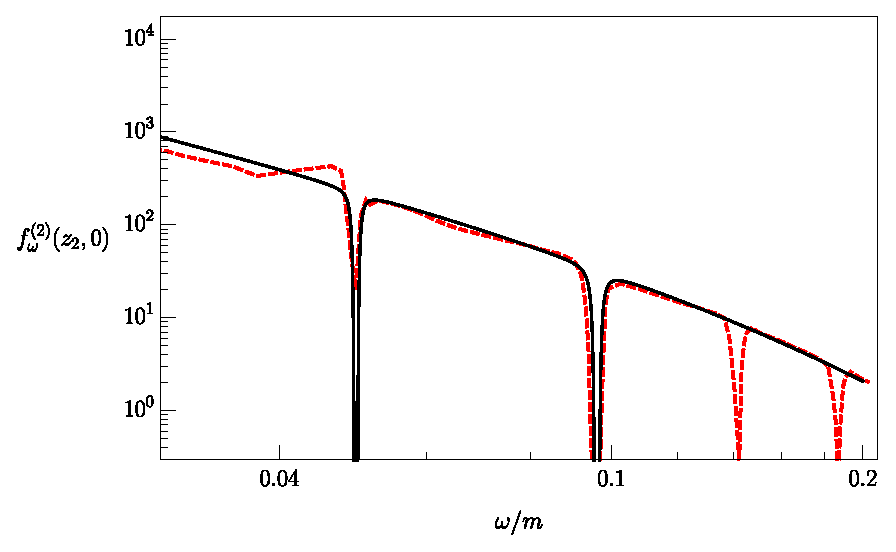
\includegraphics[width=0.7\linewidth,clip]{Fig10.eps}\\
	\caption{\label{fig:Mode22tau} Функция распределения фотона моды 2 при магнитном поле $B=0.05 B_e$ и температуре $T=3$ кэВ, для углов $\theta = 0$ ($x=0$), $\theta = \pi/3$ ($x=0.5$) и $\theta=\pi/2$ ($x=1$) между направлением импульса начального фотона и направлением магнитного поля, а также оптической толщи~$\tau_{2}=~3~\times 10^{-3}$. Штриховая линия соответствует результатам, полученным в работе~\cite{Schonherr:2007}, а сплошная линия -- дельта-функциональному приближению~(\ref{FormSolZeroL}).}
\end{figure}

Непосредственное решение системы уравнений~(\ref{eq:SysAPart}) представляет определенные вычислительные трудности в окрестности резонансов. С другой стороны, результаты, полученные в работе~\cite{Rumyantsev:2026}, показывают, что резонансный пик становится тем уже, чем меньше магнитное поле. Поэтому в относительно слабом магнитном поле $B\lesssim B_e$, с учетом узкой области резонанса и последующего интегрирования, удобно воспользоваться дельта-функциональным приближением функций $\varphi_\omega^{\lambda\lambda'}(x,x')$, т.е. относительно $x$ представить часть выражений~(\ref{eq:Varphi}), содержащую~$1/\Delta^-$, в виде:
\begin{equation}\label{eq:DeltaMDelta}
	\begin{aligned}
		\frac{1}{\Delta^-}&=\frac{1}{(\omega^2(1-x^2)+2 \omega m - 2\beta)^2 + \left(\frac{E_1^{''} \Gamma_1^\pm}{2}\right)^2}=
		\\
		&= \frac{2\pi}{E_1''\Gamma_1^-} \delta(\omega^2(1-x^2)+2 \omega m - 2\beta) + \frac{O(E_1''\Gamma_1^-)}{E_1''\Gamma_1^-}
		=
		\frac{2\pi}{E_1''\Gamma_1^-}\sum_{\sigma=\pm1}\frac{\delta(x-x_\sigma)}{2 |x_\sigma| \omega^2} + \frac{O(E_1''\Gamma_1^-)}{E_1''\Gamma_1^-} \, ,
	\end{aligned}
\end{equation} 
где 
\begin{equation}\label{eq:xi}
	x_\sigma = \sigma \sqrt{\frac{\omega^2+2\omega m - 2\beta}{\omega^2}}\, .
\end{equation}

В таком случае, учитывая только лидирующий вклад, имеем: 

\begin{equation}\label{eq:J110}
	J_\ell^{11}(\overline{s},\omega) \simeq\frac{\pi\beta^2 E_1''\Gamma_1^-}{\omega^2m^4}\sum_{\sigma=\pm1}\frac{1}{|x_\sigma|}\frac{{\cal P}_\ell(x_\sigma)}{x_\sigma \overline{s}+ 4\left(\frac{\beta^2}{m^4}+\frac{\omega^2}{3m^2}\right)} \, ,
\end{equation}
\begin{equation}\label{eq:J120}
	J_\ell^{12}(\overline{s},\omega) \simeq \frac{\pi E''_1\Gamma_1^-}{3m^2}\sum_{\sigma=\pm1}\frac{1}{|x_\sigma|} \frac{{\cal P}_\ell(x_\sigma)}{ x_\sigma\overline{s}+4\left(\frac{\beta^2}{m^4}+\frac{\omega^2}{3m^2}\right)} 
	\, ,
\end{equation}
\begin{equation}\label{eq:J220}
	J_\ell^{22}(\overline{s},\omega) \simeq\frac{\pi\omega^2 E''_1\Gamma_1^-}{3\beta m^2 }\sum_{\sigma=\pm1}\sigma \frac{{\cal P}_\ell(x_\sigma)}{\overline{s}+ 4x_\sigma \left(\frac{\omega^4}{3\beta^2 } + \frac{\omega^2}{m^2}\right)}
	\, ,
\end{equation}
\begin{equation}\label{eq:21J210}
	J_\ell^{21}(\overline{s},\omega) \simeq \frac{\pi E_1''\Gamma_1^-}{m^2}\sum_{\sigma=\pm1}\sigma \frac{{\cal P}_\ell(x_\sigma)}{\overline{s}+ 4x_\sigma \left(\frac{\omega^4}{3\beta^2 } + \frac{\omega^2}{m^2}\right)}
	\, ,
\end{equation}
где
\begin{equation}
	\overline{s}= \frac{(E_1''\Gamma_1^-)^2}{2\rho m} s\, .
\end{equation}

С учетом (\ref{eq:J110})--(\ref{eq:21J210}) выражение~(\ref{eq:SolveFunc}) можно представить в виде:
\begin{equation}\label{eq:SolveFunc2}
	f_\omega^{(\lambda)}(z, x) = \frac{1}{2\pi i}\sum_{\ell=0}^{\infty} 
	{\cal P}_\ell(x) \frac{2\rho m}{(E_1''\Gamma_1^-)^2}\int_{\overline{\sigma}_c-i\infty}^{\overline{\sigma}_c + i \infty}d\overline{s} \cdot e^{\overline{s}z/a} \overline{A}^{(\lambda)}_\ell(\overline{s},\omega)\, ,
\end{equation}
где 
\begin{equation}
	\overline{\sigma}_c= \frac{(E_1''\Gamma_1^-)^2}{2\rho m} \sigma_c\, ,
\end{equation}
а также
введен параметр размерности длины:
\begin{equation}
	a=\frac{(E_1''\Gamma_1^-)^2}{2\rho m^ 2}\, .
\end{equation}

Следует отметить, что функции~(\ref{eq:J110})--(\ref{eq:21J210}) ограничены в области 
\begin{equation}
	\sqrt{m^2+2\beta}-m<\omega<\beta/m\, ,
\end{equation}
поскольку, c одной стороны, интегрирование с дельта-функциями по переменной~$x$ происходит в ограниченных пределах $-1\leqslant x\leqslant1$, а с другой стороны, подкоренное выражение в~(\ref{eq:xi}) должно быть положительным, иначе требуется следующий порядок разложения в дельта-функциональном приближении. В качестве иллюстрации решения~(\ref{eq:SolveFunc2}) c учетом дельта-функциональной аппроксимации резонансного пика выберем величины магнитного поля $B=0.05 B_e$ и~температуры $T\simeq11$~кэВ. Для данных значений параметров среды циклотронный резонанс имеет место на энергиях фотона $\omega\sim T\simeq11$ кэВ, а ширина резонанса с увеличением температуры уменьшается. В качестве граничного условия при $z=0$ выберем равновесную функцию распределения фотонов:
\begin{equation}
	f_{0\omega} = \frac{1}{\exp[\omega/T]-1}.
\end{equation}

 Введем спектральную плотность распределения энергии фотонов согласно~\cite{Landau:2002}:
\begin{equation}\label{eq:PowerSpectra}
	R_\omega^{(\lambda)}(z, x)=\frac{\omega^3}{4\pi^3} f_\omega^{(\lambda)}(z, x)
\end{equation}
и будем полагать, что только комптоновский процесс в резонансной области энергий фотона вносит изменение в функцию распределения. Поэтому  в нерезонансных областях $0\leqslant\omega <\sqrt{m^2+2\beta}-m$ и $\omega>\beta/m$ коэффициенты $\overline{A}^{(\lambda)}_\ell(\overline s,\omega)$ с~учетом граничного условия~(\ref{eq:GranS}) примут вид:
\begin{equation}
	\overline{A}_0^{(\lambda)}(\overline{s},\omega)=\frac{(E_1''\Gamma_1^-)^2}{2\rho m}\frac{f_{0\omega}}{\overline{s}},
\end{equation}
\begin{equation}
	\overline{A}_\ell^{(\lambda)}(\overline{s},\omega)=0, \, \, \ell>0.
\end{equation}

В резонансной области уравнение~(\ref{eq:SysAPart}) решалось для дискретных значений $\textrm{Im}(\overline{s})$ для интервала $-10^3<\textrm{Im}(\overline{s})<10^3$ с шагом дискретизации $\Delta \overline{s}=0.1$. Значение действительной части переменной $\overline{s}$ выбиралось так, чтобы все полюса выражений~(\ref{eq:J110})--(\ref{eq:21J210}) на комплексной плоскости находились левее $\text{Re} \overline{s}=\overline{\sigma}_c$, где $\text{Re} \overline{s}$ определяется неравенствами:
\begin{equation}\begin{gathered}\label{eq:condw}
		\textrm{Re }\overline{s}>4\left(\frac{\beta^2}{m^4}+\frac{\omega^2}{3m^2}\right),\\
		\textrm{Re }\overline{s}>4 \left(\frac{\omega^4}{3\beta^2 } + \frac{\omega^2}{m^2}\right).
	\end{gathered}	
\end{equation}

При этом выбор реальной части в виде $\textrm{Re }\overline{s}=1$ заведомо удовлетворяет условиям~(\ref{eq:condw}).
Проведенный численный анализ уравнения~(\ref{eq:SysAPart}) показал, что коэффициенты $\overline{A}^{(\lambda)}_\ell(s,\omega)$ при $\ell>2$ имеют пренебрежимо малые значения для обеих мод фотона $\lambda=1,2$.


%На рис.~\ref{fig:Transf2zkx120cm}--\ref{fig:Transf2zkx240cm2} представлены численные результаты для зависимости  спектральной плотности~(\ref{eq:PowerSpectra}) от энергии фотона вблизи резонанса в сравнении со спектральной плотности излучения черного тела:
%\begin{equation}\label{eq:BlackPowerSpectra}
%	R_0(\omega)=\frac{\omega^3}{4\pi^3} \frac{1}{\exp[\omega/T]-1}\, ,
%\end{equation}
%для различных значений высоты $z$ колонки вещества и угла $\theta$ между направлением импульса фотона и направлением магнитного поля как для моды 1, так и~для~моды~2. Из предположения дипольной конфигурации магнитного поля, которая является достаточно хорошим приближением вблизи полярной шапки~\cite{Thompson:1995}, следует, что магнитное поле можно считать постоянным и однородным в масштабах сотен метров.
%
%Для магнитного поля $B=10^{12}$ Гс на масштабе $z\simeq a$ как для фотона моды~1, так и для фотона моды~2 имеются незначительные изменения спектра по сравнению со спектром излучения черного тела, даже вблизи границы резонансной области $\omega\simeq 11$ кэВ. С увеличением масштаба до значений $z\simeq 5a$ наблюдается увеличение спектральной плотности  на 7\% при всех энергиях начального фотона (см. рис.~\ref{fig:Transf1zkx120cm2}). При значениях  $z\simeq 10 a$ резонансный комптоновский процесс приводит к значительному уменьшению спектральной плотности  во всей резонансной области. Отметим, что спектр для фотона моды 1 практически не зависит от угла импульса фотона по отношению к магнитному полю.
%
%Несколько иная ситуация наблюдается для спектра излучения фотонов моды 2 (см. рис.~\ref{fig:Transf2zkx120cm}--~\ref{fig:Transf2zkx240cm2}). Анализ полученных результатов позволяет заключить, что спектр для фотона моды~2 существенно отличается во всей резонансной области от спектра излучения черного тела для масштаба $z\gtrsim 5a$.  Вблизи порога резонансной области $\omega\simeq 11$~кэВ для фотонов, которые распространяются под углами, близкими к направлению магнитного поля, спектр имеет заниженные значения по сравнению со спектром излучения черного тела. С другой стороны, отмечается превышение спектра в околопороговой области для фотонов, распространяющихся в направлении, перпендикулярном магнитному полю. Однако, в отличие от спектра моды 1, уже на масштабах $z\simeq5a$ наблюдается заметное увеличение спектральной плоскости в более низкоэнергетической части рассматриваемой области.
%Также следует отметить, что спектр фотона моды~2 в этой области начинает существенно зависеть от угла между направлением импульса фотона и направлением магнитного поля. При значении $z\simeq 10 a$ спектральная плотность во всей области резонанса существенно меньше, чем спектральная плотность излучения черного тела.
%Для фотонов, распространяющихся вдоль магнитного поля, существуют области энергий, при которых дельта-функциональное приближение~(\ref{eq:DeltaMDelta}) неприменимо, что требует отдельного исследования.	

%\begin{figure}\centering
%	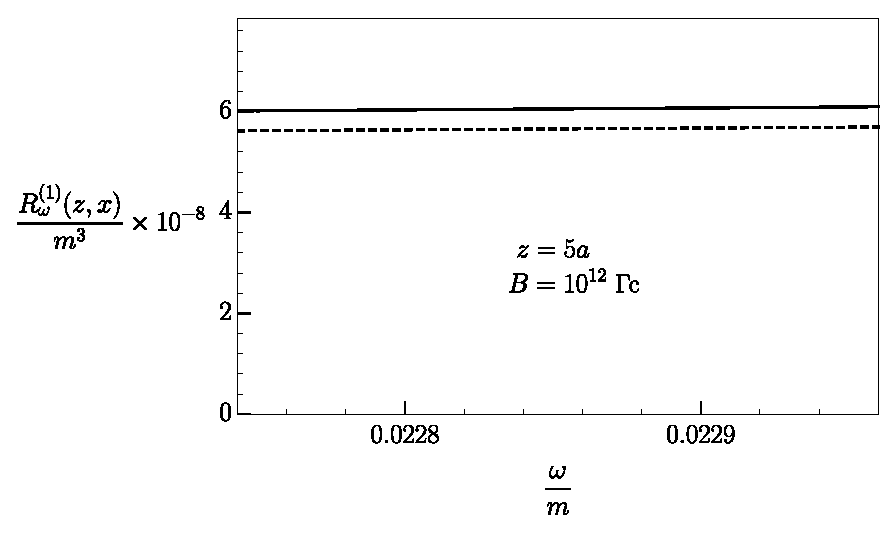
\includegraphics[width=1\linewidth,clip]{Fig11.eps}
%	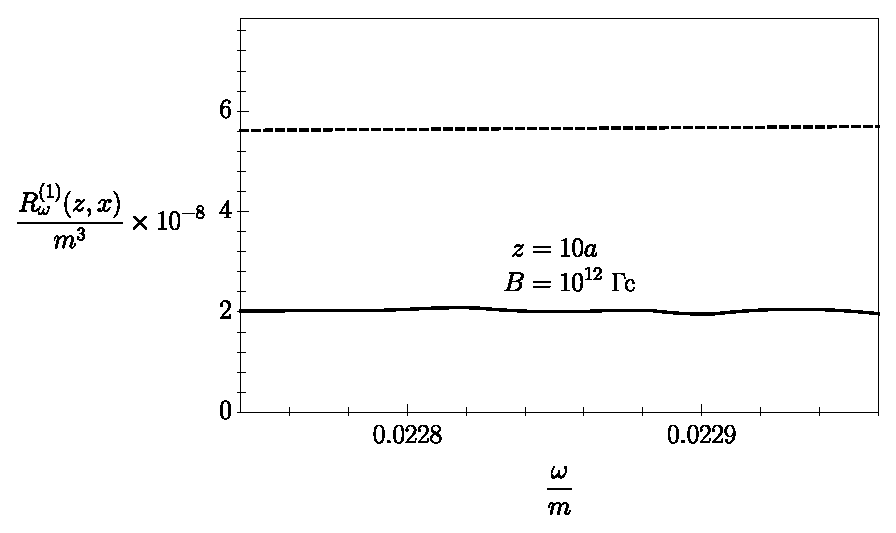
\includegraphics[width=1\linewidth,clip]{Fig12.eps}
%	\caption{Спектральная плотность~(\ref{eq:PowerSpectra}) моды 1 с учетом резонансного комптоновского процесса для произвольного угла между направлением импульса начального фотона и направлением магнитного поля. Штриховая линия --  спектральная плотность  чернотельного излучения~(\ref{eq:BlackPowerSpectra}). }\label{fig:Transf1zkx120cm2}
%\end{figure}
%
%\begin{figure}\centering
%	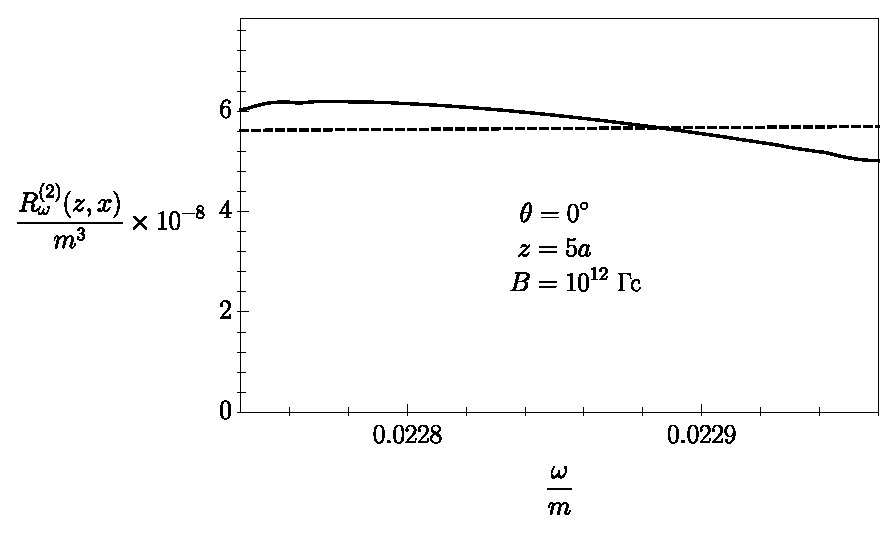
\includegraphics[width=1\linewidth,clip]{Fig13.eps}	\\
%	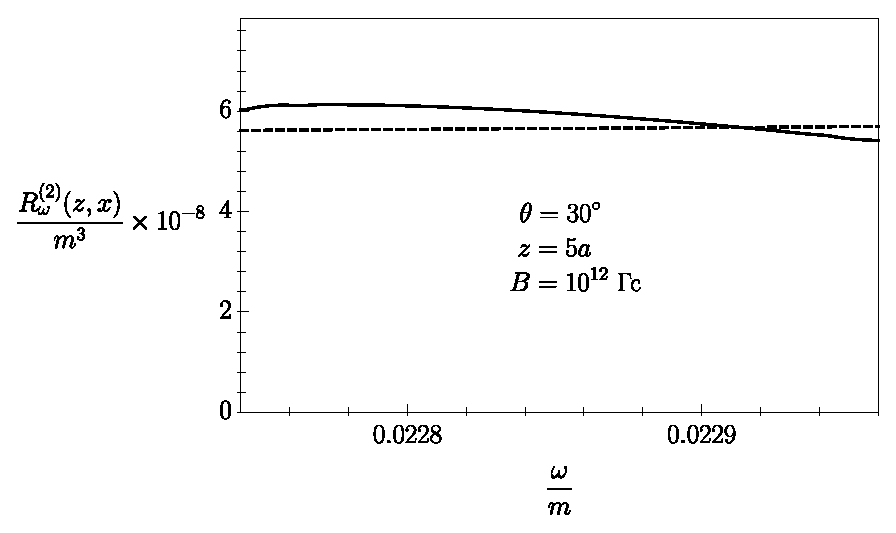
\includegraphics[width=1\linewidth,clip]{Fig14.eps}
%	\caption{Спектральная плотность~(\ref{eq:PowerSpectra}) моды 2 с учетом резонансного комптоновского процесса. Штриховая линия --  спектральная плотность  чернотельного излучения~(\ref{eq:BlackPowerSpectra})}\label{fig:Transf2zkx120cm}
%\end{figure}
%
%\begin{figure}\centering
%	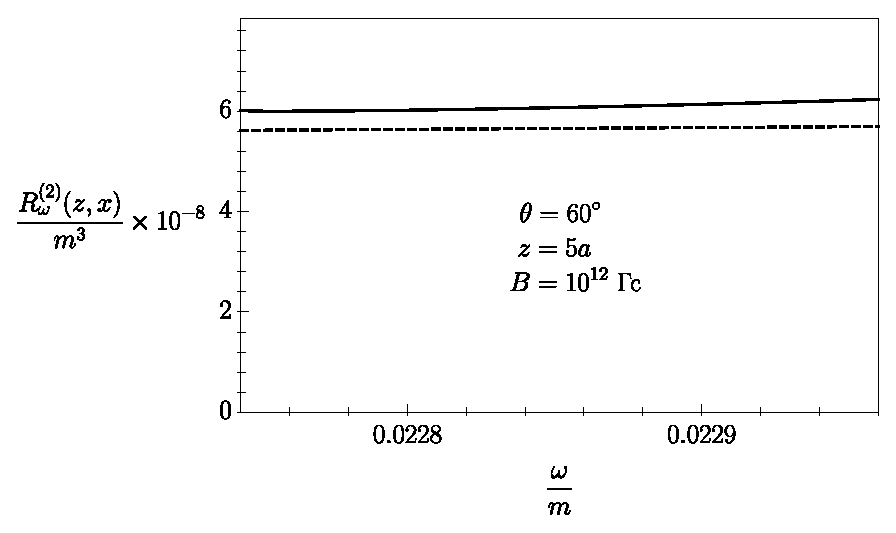
\includegraphics[width=1\linewidth,clip]{Fig15.eps}	\\
%	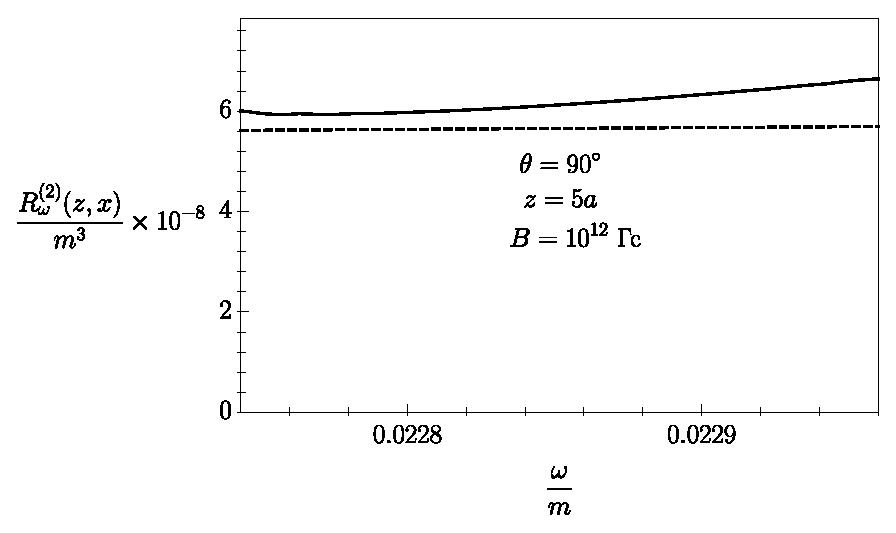
\includegraphics[width=1\linewidth,clip]{Fig16.eps}
%	\caption{Спектральная плотность~(\ref{eq:PowerSpectra}) моды 2 с учетом резонансного комптоновского процесса. Штриховая линия --  спектральная плотность  чернотельного излучения~(\ref{eq:BlackPowerSpectra})}\label{fig:Transf2zkx120cm2}
%\end{figure}
%
%\begin{figure}\centering
%	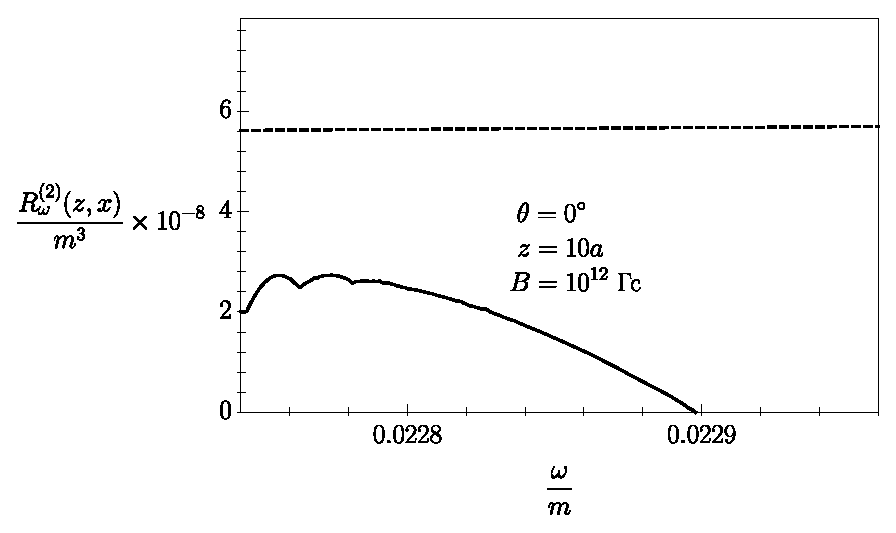
\includegraphics[width=1\linewidth,clip]{Fig17.eps}	\\
%	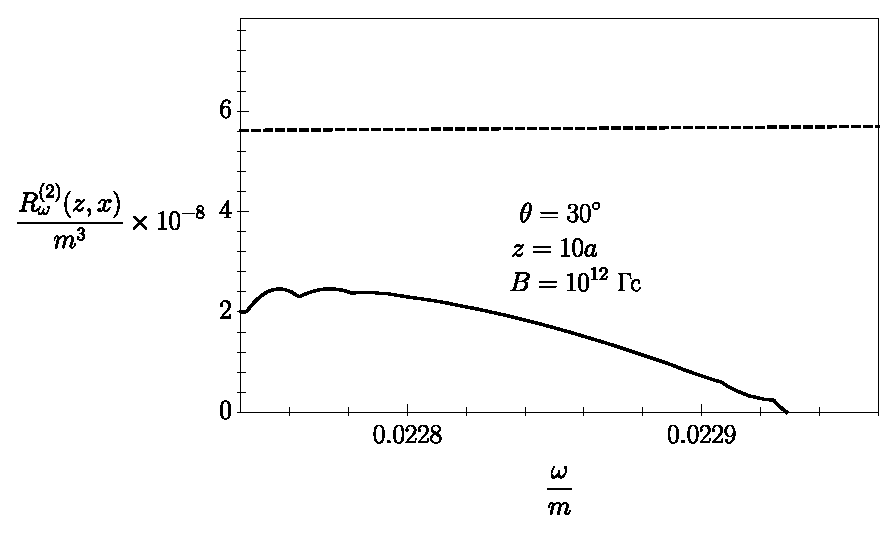
\includegraphics[width=1\linewidth,clip]{Fig18.eps}
%	\caption{Спектральная плотность~(\ref{eq:PowerSpectra}) моды 2 с учетом резонансного комптоновского процесса. Штриховая линия --  спектральная плотность  чернотельного излучения~(\ref{eq:BlackPowerSpectra})}\label{fig:Transf2zkx240cm}
%\end{figure}
%
%\begin{figure}\centering
%	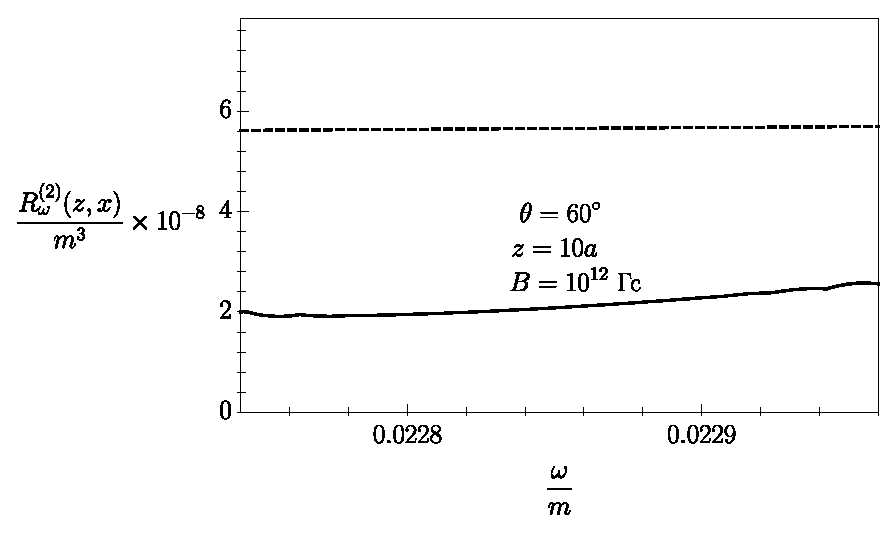
\includegraphics[width=1\linewidth,clip]{Fig19.eps}	\\
%	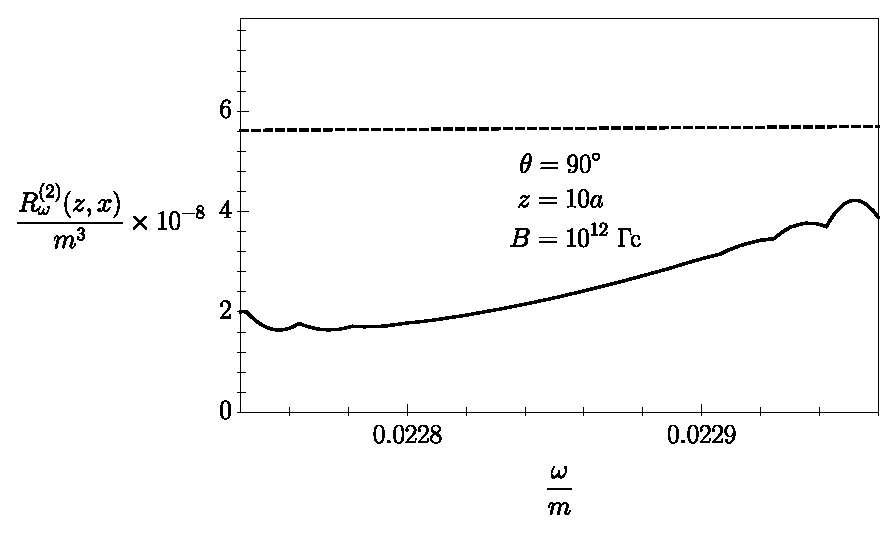
\includegraphics[width=1\linewidth]{Fig20.eps}
%	\caption{Спектральная плотность~(\ref{eq:PowerSpectra}) моды 2 с учетом резонансного комптоновского процесса. Штриховая линия --  спектральная плотность  чернотельного излучения~(\ref{eq:BlackPowerSpectra})}\label{fig:Transf2zkx240cm2}
%\end{figure}	

%%%%%%%%%%%%%%%%%%%%%%%%%%%%%%%%%%%%%%%%%%%%%%%%%%%%%%%%%%%%%%%%%%%%%%%%%%%%%%%%%%%%%%%%%%%%%%%%%%%%%%%%%%%%%%%%%%%%%%%%%%%%%%%%%%%%%%%%%%%%%%%%%%%%%%%%%%%
\section{Заключение}

Рассмотрено решение кинетического уравнения для нахождения функции распределения фотонов двух возможных поляризаций в равновесной нерелятивистской плазме электронов в относительно сильном магнитном поле с учетом резонанса на виртуальном электроне.
Используя преобразование Лапласа и разложение функции распределения по полиномам Лежандра задача сведена к решению системы дифференциальных уравнений на определение коэффициентов этого разложения. Решение представлено в виде интеграла в комплексной плоскости. Для значения магнитного поля $B\simeq10^{12}$ Гс и $T\simeq11$ кэВ вычислена спектральная плотность распределения энергии излучения. Показано, что для фотона моды~1 в резонансной области при $z\lesssim a$ спектр практически совпадает с чернотельным спектром, в то время как для моды 2 спектр претерпевает существенные изменения. Это может говорить о том что мода 1 при таких условиях практически все время будет находиться в состоянии равновесия, тогда как поведение фотона моды 2 носит существенно неравновесный характер. Данный вывод согласуется с результатами предыдущих исследований (см., например,~\cite{Lubarsky:1988}). Для масштабов расстояний $z\gtrsim a$, модификация спектра как для фотона моды 2, так и для фотона моды 1 становится существенной. Изменения становятся особенно значительны для фотонов моды 2, распространяющихся вдоль магнитного поля, что требует отдельного исследования правомочности использования как дельта-функционального приближения~(\ref{eq:DeltaMDelta}), так и преобразования Лапласа~(\ref{eq:SolveFunc}) на границе резонансной области.

Полученные результаты могут быть использованы для построения спектра излучения аккреционной колонки электронной плазмы. Для этого, согласно работе~\cite{Nishimura:2008} можно разделить аккреционную колонку на малые области с постоянным значением магнитного поля и температуры, а результирующий спектр может быть найден как сумма резонансных вкладов от этих областей.
%%%%%%%%%%%%%%%%%%%%%%%%%%%%%%%%%%%%%%%%%%%%%%%%%%%%%%%%%%%%%%%%%%%%%%%%%%%%%%%%%%%%%%%%%%%%%%%%%%%%%%

\section*{Приложение 1.}

\begin{center}
	\textbf{Амплитуды поглощения фотона}
\end{center}


Входящие в выражение~(\ref{eq:amplonever}) величины ${\cal T}^{s'' s}_\lambda$ выражаются через следующие 
лоренц-инварианты относительно преобразований вдоль направления магнитного поля:
%
\begin{eqnarray}
	\label{eq:K1}
	&&{\cal K}_{1}^{(\lambda)} = \sqrt{\frac{2}{(p\tilde \varphi\tilde \varphi p^{\, \prime \prime}) + 
			M_\ell M_{n}}} \times 
	\\
	\nonumber 
	&&\times \left \{M_\ell (\varepsilon^{(\lambda)}\tilde \varphi\tilde \varphi p^{\, \prime \prime}) + 
	M_{n} (\varepsilon^{(\lambda)}\tilde \varphi\tilde \varphi p)  \right \}\, ,
\end{eqnarray}
%
\begin{eqnarray}
	&&{\cal K}_{2}^{(\lambda)} = \sqrt{\frac{2}{(p\tilde \varphi\tilde \varphi p^{\, \prime \prime}) + 
			M_\ell M_{n}}} 
	\times
	\\
	\nonumber
	&&\times
	\left \{M_\ell (\varepsilon^{(\lambda)}\widetilde \varphi p^{\, \prime \prime}) + 
	M_{n} (\varepsilon^{(\lambda)}\widetilde \varphi p)  \right \}\, ,
	\label{eq:K2}
\end{eqnarray}
%
\begin{eqnarray}
	{\cal K}_{3} = \sqrt{2\left [(p\tilde \varphi\tilde \varphi p^{\, \prime \prime}) + 
		M_\ell M_{n} \right]} \, ,  
\end{eqnarray}
%
\begin{eqnarray}
	{\cal K}_4 = 
	- \sqrt{\frac{2}{(p\tilde \varphi\tilde \varphi p^{\, \prime \prime}) + M_\ell M_{n}}}\, 
	(p\widetilde \varphi p^{\, \prime \prime}) \, ,
	\label{eq:K34}
\end{eqnarray}
%

Выражения для ${\cal T}^{s'' s}_\lambda$ могут быть получены из~\cite{Rumyantsev:2017} и представлены в виде:
%
\begin{eqnarray}
	\nonumber
	&&{\cal T}^{--}_\lambda  = e [ 2\beta\sqrt{\ell n} {\cal K}_1^{(\lambda)} I_{n-1,\ell-1} +
	\\[3mm]
	\label{eq:tV--}
	&&+ (M_\ell + m)(M_n + m) {\cal K}_1^{(\lambda)} I_{n,\ell} -
	\\[3mm]
	\nonumber
	%transversal
	&&-\sqrt{2\beta n} (M_\ell + m) {\cal K}_3 \times
	\\[3mm]
	\nonumber
	&&\times\frac{(\varepsilon^{(\lambda)}\varphi\varphi q) - 
		\ii (\varepsilon^{(\lambda)} \varphi q)}{\sqrt{q^2_{\mprp}}} I_{n-1,\ell} -
	\\[3mm]
	\nonumber
	&&- \sqrt{2\beta \ell} (M_n + m) {\cal K}_3 \times
	\\[3mm]
	\nonumber
	&&\times
	\frac{(\varepsilon^{(\lambda)}\varphi\varphi q) + \ii (\varepsilon^{(\lambda)}\varphi q)}{\sqrt{q^2_{\mprp}}} I_{n,\ell-1}] \, ,
\end{eqnarray}



\begin{eqnarray}
	\nonumber
	&&{\cal T}^{-+}_\lambda = \ii e [\sqrt{2\beta n} (M_\ell + m) {\cal K}_2^{(\lambda)} 
	I_{n-1,\ell-1} - 
	\\[3mm]\nonumber
	&&- \sqrt{2\beta \ell} (M_n + m) {\cal K}_2^{(\lambda)} 
	I_{n,l} +
	\\[3mm]
	\nonumber
	%transversal
	&&+ 2\beta\sqrt{\ell n} {\cal K}_4 
	\frac{(\varepsilon^{(\lambda)}\varphi\varphi q) - \ii (\varepsilon^{(\lambda)}\varphi q)}{\sqrt{q^2_{\mprp}}} I_{n-1,\ell} -
	\nonumber\\[3mm]
	&&- (M_\ell + m)(M_n + m) {\cal K}_4 \times
	\\[3mm]
	\nonumber
	&&\times
	\frac{(\varepsilon^{(\lambda)}\varphi\varphi q) + \ii (\varepsilon^{(\lambda)}\varphi q)}{\sqrt{q^2_{\mprp}}} I_{n,\ell-1}]  \, ,
	\nonumber
\end{eqnarray}

\begin{eqnarray}
	&&{\cal T}^{+-}_\lambda = -\ii e [\sqrt{2\beta \ell} (M_n + m) {\cal K}_2^{(\lambda)} 
	I_{n-1,\ell-1} - 
	\nonumber\\[3mm]
	&&- \sqrt{2\beta n} (M_\ell + m) {\cal K}_2^{(\lambda)} 
	I_{n,\ell} +
	\\[3mm]
	\nonumber
	%transversal
	&&+ (M_\ell + m)(M_n + m) {\cal K}_4 \times
	\\[3mm]
	\nonumber
	&&\times
	\frac{(\varepsilon^{(\lambda)}\varphi\varphi q) - \ii (\varepsilon^{(\lambda)}\varphi q)}{\sqrt{q^2_{\mprp}}} I_{n-1,\ell} -
	\nonumber\\[3mm]
	&&- 2\beta\sqrt{\ell n} {\cal K}_4 
	\frac{(\varepsilon^{(\lambda)}\varphi\varphi q) + \ii (\varepsilon^{(\lambda)}\varphi q)}{\sqrt{q^2_{\mprp}}} I_{n,\ell-1}]  \, ,
	\nonumber
\end{eqnarray}

\begin{eqnarray}
	\nonumber
	&&{\cal T}^{++}_\lambda  = e [2\beta\sqrt{\ell n} {\cal K}_1^{(\lambda)} I_{n,\ell} +
	\\[3mm]
	\label{eq:tV++} 
	&&+ (M_\ell + m)(M_n + m) {\cal K}_1^{(\lambda)} I_{n-1,\ell-1} -
	\\[3mm]
	\nonumber
	%transversal
	&&- \sqrt{2\beta \ell} (M_n + m) {\cal K}_3 \times
	\\[3mm]
	\nonumber
	&&\times
	\frac{(\varepsilon^{(\lambda)}\varphi\varphi q) - \ii (\varepsilon^{(\lambda)}\varphi q)}{\sqrt{q^2_{\mprp}}} I_{n-1,\ell} -
	\\[3mm]
	\nonumber
	&&- \sqrt{2\beta n} (M_\ell + m) {\cal K}_3 \times
	\\[3mm]
	\nonumber
	&&\times
	\frac{(\varepsilon^{(\lambda)}\varphi\varphi q) + \ii (\varepsilon^{(\lambda)}\varphi q)}{\sqrt{q^2_{\mprp}}} I_{n,\ell-1}] \, .
\end{eqnarray}
%%%%%%%%%%%%%%%%%%%%%%%%%%%%%%%%%%%%%%%%%%%%%%%%%%%%%%%%%%%%%%%%%%%%%%%%
%% Библиография %%%%%%%%%%%%%%%%%%%%%%%%%%%%%%%%%%%%%%%%%%%%%%%%%%%%%%%%
%%%%%%%%%%%%%%%%%%%%%%%%%%%%%%%%%%%%%%%%%%%%%%%%%%%%%%%%%%%%%%%%%%%%%%%%

\bibliographystyle{plain}
\begin{thebibliography}{}

\bibitem{Nagel:1981}
Nagel W. Radiative transfer in a strongly magnetized plasma. I - Effects of
anisotropy. II - Effects of Comptonization // Astrophys. J. 1981. Vol. 251.
P. 278–296.
%
\bibitem{Kaminker:1982}
Kaminker A. D., Pavlov G. G., Shibanov Y. A. Radiation from a stronglymagnetized
plasma: the case of predominant scattering // Astrophys. Space
Sci. 1982. Vol. 86, no. 2. P. 249–297.
%
\bibitem{Alexander:1991}
Alexander S. G., Meszaros P. Cyclotron Harmonics in Accreting Pulsars and
Gamma-Ray Bursters: Effect of Two-Photon Processes // Astrophys. J. 1991.
Vol. 372. P. 565–572.
%
\bibitem{Meszaros:1985}
Meszaros P., Nagel W. X-ray pulsar models. II. Comptonized spectra and pulse
shapes. // Astrophys. J. 1985. Vol. 299. P. 138–153.
%
\bibitem{Nishimura:2008}
Nishimura O. Formation Mechanism for Broad and Shallow Profiles of Cyclotron
Lines in Accreting X-Ray Pulsars // Astrophys. J. 2008. Vol. 672,
no. 2. P. 1127–1136.
%
\bibitem{Mihalas:1985}
Mihalas D. The computation of radiation transport using feautrier variables I.
Static media // J. Comput. Phys. 1985. Vol. 57, no. 1. P. 1–25.
%
\bibitem{Yahel:1979}
Yahel R. Z. Cyclotron line formation in the atmosphere of a mgnetized neutron 
star // Astrophys. J. Lett. 1979. Vol. 229. P. 73–79.
%
\bibitem{Araya:1999}
Araya R. A., Harding A. K. Cyclotron Line Features from Near-critical Magnetic
Fields: The Effect of Optical Depth and Plasma Geometry // Astrophys.
J. 1999. Vol. 517, no. 1. P. 334–354.
%
\bibitem{Nobili:2008}
Nobili L., Turolla R., Zane S. X-ray spectra from magnetar candidates –
II. Resonant cross-sections for electron–photon scattering in the relativistic
regime // Mon. Not. Roy. Astron. Soc. 2008. Vol. 389, no. 2. P. 989–1000.
%
\bibitem{Fernandez:2011}
Fernandez R., Davis S. W. The X-ray polarization signature of quiescent magnetars:
effect of magnetospheric scattering and vacuum polarization // Astrophys.
J. 2011. Vol. 730, no. 131. P. 21.
%
\bibitem{Taverna:2014}
Taverna R., Muleri F., Turolla R. et al. Probing magnetar magnetosphere
through X-ray polarization measurements // Mon. Not. Roy. Astron. Soc.
2014. Vol. 438, no. 2. P. 1686–1697.
%
\bibitem{Mustukov:2021}
Mushtukov A. A., Suleimanov V. F., Tsygankov S. S., Portegies Zwart S. Spectrum
formation in X-ray pulsars at very low mass accretion rate: Monte Carlo
approach // Mon. Not. Roy. Astron. Soc. 2021. Vol. 503, no. 4. P. 5193–5203.
%
\bibitem{Mushtukov:2022}
Mushtukov A., Markozov I., Suleimanov V. et al. Statistical features of multiple
Compton scattering in a strong magnetic field // Phys. Rev. D. 2022. Vol.
105, no. 10. P. 103027.
%
\bibitem{Fernandez:2007}
Fernandez R., Thompson C. Resonant Cyclotron Scattering in Three Dimensions and the Quiescent Nonthermal X-ray Emission of Magnetars // Astrophys.~J. 2007 Vol. 660. no. 1. P. 615--640.
%
\bibitem{Caflisch:1998}
Caflisch R. E. Monte Carlo and quasi-Monte Carlo methods // Acta Numerica.
1998. Vol. 7. P. 1–49.
%
\bibitem{Hall:2009}
Hall M. G., Alexander D. C. Convergence and Parameter Choice for MonteCarlo
Simulations of Diffusion MRI // IEEE Transactions on Medical Imaging.
2009. Vol. 28, no. 9. P. 1354–1364.
%
\bibitem{Meszaros:1983}
Meszaros P., Harding A. K., Kirk J. G., Galloway D. J. Accreting X-ray pulsar
atmospheres heated by Coulomb deceleration of protons // Astrophys. J. Lett.
1983. Vol. 266. P. 33–37.
%
\bibitem{Harding:1984}
Harding A. K., Meszaros P., Kirk J. G., Galloway D. J. Self-consistent models
for Coulomb-heated X-ray pulsar atmospheres. // Astrophys. J. 1984. Vol. 278.
P. 369–381.
%
\bibitem{Nishimura:2015}
Nishimura O. Properties of cyclotron lines in a line-forming region injected by
an anisotropic continuum in accreting X-ray pulsars // Astrophys. J. 2015.
Vol. 807, no. 164. P. 14.
%
\bibitem{Basko:1976}
Basko M. M., Sunyaev R. A. The limiting luminosity of accreting neutron
stars with magnetic fields. // Mon. Not. Roy. Astron. Soc. 1976. Vol. 175.
P. 395–417.
%
\bibitem{YarkovPhotFE:2023}
Ярков A.~A., Румянцев Д.~A. Решение кинетического уравнения с учетом резонанса в комптоновском процессе в замагниченной среде. // Письма в журнал Физика элементарных частиц и атомного ядра. 2023. Т. 20. № 3(248). С. 422--427.
%
\bibitem{Rumyantsev:2017}
Румянцев Д. А., Шленев Д. М., Ярков А. А. // ЖЭТФ 152, 483 (2017).
%
\bibitem{Gradstein:1963}
Градштейн И. С., Рыжик И. М., Таблицы инте-
гралов, сумм, рядов и произведений, Физматлит:
Москва (1963).
%
\bibitem{Kompaneets:1957}
Kompaneets A.S. The Establishment of Thermal Equilibrium between Quanta and Electrons // JETP. 1957. Vol. 4. P. 730.
%
\bibitem{Lubarsky:1988}
Lyubarskii, Yu. E. Comptonization in a superstrong magnetic field. I. // Astrophysics (Engl. Transl.). 1988. Vol. 28:1.
%
\bibitem{Kuznetsov:2003}
Kuznetsov A. V., Mikheev N. V. Electroweak processes in external electromagnetic
fields. New York: Springer-Verlag, 2003. 120 p.
%
\bibitem{Schonherr:2007}
Sch	onherr G., Wilms J., Kretschmar P. et al. A model for cyclotron resonance
scattering features // Astronomy \& Astrophysics. 2007. Vol. 472, no. 2.
P. 353–365.
%
\bibitem{SandeepK:2022}
Kumar S., Bala S., Bhattacharya D. A new Monte Carlo radiative transfer
simulation of cyclotron resonant scattering features // Mon. Not. Roy. Astron.
Soc. 2022. Vol. 515, no. 1. P. 914–927.
%
\bibitem{Thompson:1995}
Thompson C., Duncan R. C. The soft gamma repeaters as very strongly magnetized
neutron stars - I. Radiative mechanism for outbursts // Mon. Not.
Roy. Astron. Soc. 1995. Vol. 275. P. 255–300.
%
\bibitem{Rumyantsev:2026}
Румянцев Д. А., Шленев Д. М., Ярков А. А. // ЖЭТФ ?, ? (2026).
%
\bibitem{Landau:2002}
Ландау Л. Д., Лифшиц Е. М. Теоретическая физика: ч. 1. Статистическая
физика. Теория конденсированного состояния. ФИЗМАТЛИТ, 2002. Т. V.
616 с.


\end{thebibliography}

\end{document}






